\documentclass[]{spie}  %>>> use for US letter paper
%%\documentclass[a4paper]{spie}  %>>> use this instead for A4 paper
%%\documentclass[nocompress]{spie}  %>>> to avoid compression of citations
%% \addtolength{\voffset}{9mm}   %>>> moves text field down
%% \renewcommand{\baselinestretch}{1.65}   %>>> 1.65 for double spacing, 1.25 for 1.5 spacing 
%  The following command loads a graphics package to include images 
%  in the document. It may be necessary to specify a DVI driver option,
%  e.g., [dvips], but that may be inappropriate for some LaTeX 
%  installations. 
\usepackage[]{graphicx}
\usepackage{float}
\usepackage{subcaption}
\usepackage{amsmath}
\usepackage{enumitem}
\usepackage{multicol}
\usepackage{cleveref}
\usepackage{hyperref}
\usepackage{wrapfig}
%\usepackage[utf8]{inputenc}
%\usepackage[english]{babel}
%\usepackage{chngcntr}
%\usepackage{hyperref}
%\usepackage[export]{adjustbox}[2011/08/13]
%\usepackage[round]{natbib}
%\usepackage{booktabs}
%\usepackage{listings}
%\usepackage{titlesec}
%\usepackage{textcomp}




\graphicspath{{./images/}}

\title{FADTTSter: Accelerating Hypothesis Testing With Functional Analysis of Diffusion Tensor Tract Statistics} 

\author{Jean Noel\supit{1}, Juan C. Prieto\supit{1} and Martin Styner\supit{1}
\skiplinehalf
\supit{1}Neuro Image Research and Analysis Laboratory, Department of Psychiatry,\\University of North Carolina, Chapel Hill, NC, USA
}

%>>>> Further information about the authors, other than their 
%  institution and addresses, should be included as a footnote, 
%  which is facilitated by the \authorinfo{} command.

\authorinfo{Further author information:\\J.C.P.: E-mail: jprieto@med.unc.edu\\J.N.: E-mail:jeantm@email.unc.edu\\M.S.: styner@cs.unc.edu\\Send correspondence to J.C.P.
}
%%>>>> when using amstex, you need to use @@ instead of @
 

%%%%%%%%%%%%%%%%%%%%%%%%%%%%%%%%%%%%%%%%%%%%%%%%%%%%%%%%%%%%% 
%>>>> uncomment following for page numbers
\pagestyle{plain}  
%>>>> uncomment following to start page numbering at xxx
%\setcounter{page}{xxx} 
 
\begin{document} 
\maketitle 

%%%%%%%%%%%%%%%%%%%%%%%%%%%%%%%%%%%%%%%%%%%%%%%%%%%%%%%%%%%%% 
\begin{abstract}

Functional Analysis of Diffusion Tensor Tract Statistics (FADTTS) 
is a toolbox for analysis of white matter (WM) fiber tracts. 
It allows associating diffusion properties along major WM bundles 
with a set of covariates of interest, such as age, diagnostic status and gender, 
and the structure of the variability of these WM tract 
properties.

However, to use this toolbox, a user must have an intermediate knowledge in scripting languages (MATLAB). 
FADTTSter was created to overcome this issue and make the statistical analysis accessible to any 
non-technical researcher. FADTTSter is actively being used by researchers at the University of North Carolina. 
FADTTSter guides non-technical users through a series of steps including quality control of subjects and fibers in order
to setup the necessary parameters to run FADTTS. 

Additionally, FADTTSter implements interactive charts for FADTTS' outputs. This interactive chart enhances 
the researcher experience and facilitates the analysis of the results. 
FADTTSter's motivation is to improve usability and provide a new analysis tool to the community that complements FADTTS.

Ultimately, by enabling FADTTS to a broader audience, FADTTSter seeks to accelerate hypothesis testing in neuroimaging studies involving heterogeneous clinical data and diffusion tensor imaging.

This work is submitted to the Biomedical Applications in Molecular, Structural, and Functional Imaging conference. 
The source code of this application is available in NITRC\footnote{\url{http://www.nitrc.org/namicdtifiber/}}.

\end{abstract}

%>>>> Include a list of keywords after the abstract 
\keywords{FADTTS, statistical analysis, diffusion tensor imaging, diffusion profile, Matlab}

%%%%%%%%%%%%%%%%%%%%%%%%%%%%%%%%%%%%%%%%%%%%%%%%%%%%%%%%%%%%%
\section{INTRODUCTION}
\label{sec:intro}

Diffusion Tensor Imaging (DTI) has become a standard for the analysis of normal brain development and brain pathologies.
DTI measures the diffusion of water molecules which is isotropic in cell bodies and spinal fluids, and anisotropic 
in axons comprising the white matter (WM) \cite{feldman2010diffusion}. 
These characteristics allows mapping and visualizing the WM fiber tracts in the brain \cite{dti_brain_mapping1_article,dti_brain_mapping2_article} and enables assessing WM fiber integrity.

\begin{wrapfigure}{L}{0.3\textwidth}
	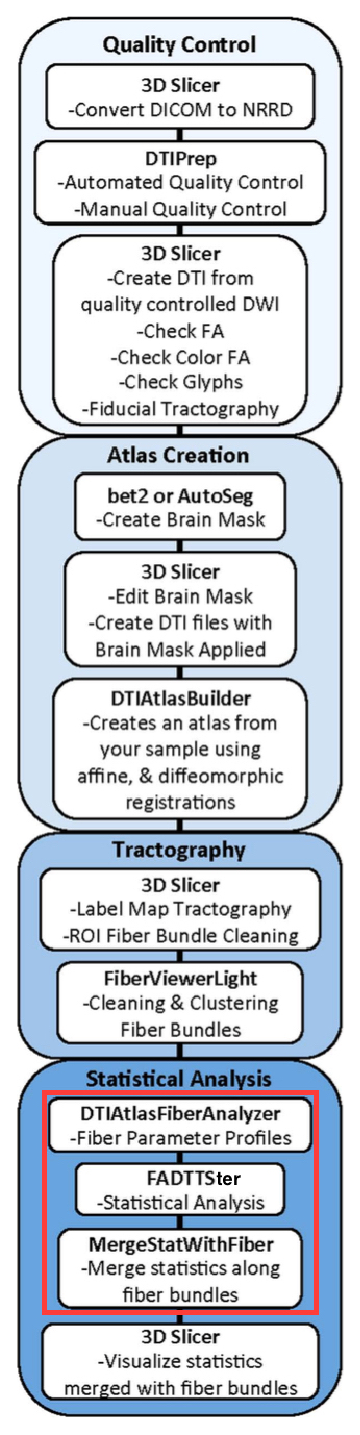
\includegraphics[width=0.27\textwidth]{namicFrameworkOut.eps}
	\caption[NA-MIC framework]{FADTTSter in the UNC-Utah NA-MIC DTI framework}
	\label{fig:namicFramework}  
	\vspace{-60pt}
\end{wrapfigure}

Functional Analysis of Diffusion Tensor Tract Statistics (FADTTS) is a tool developed to outline the evolution of diffusion properties such as axial diffusivity (AD), radial diffusivity (RD), mean diffusivity (MD) and fractional anisotropy (FA) along white matter fiber tracts and their correlation with a set of covariates of interest, such as age or gender \cite{fadtts_article}. The tool is used to facilitate the understanding of normal brain development, the neural bases of neuropsychiatric disorders, and the joint effects of environmental and genetic factors on white matter fiber bundles. 
FADTTS is capable of modeling the structured inter-subject variability, test joint effects, and construct simultaneous confidence bands. 

FADTTS is embedded in the UNC-Utah NAMIC DTI framework, an end-to-end toolbox for atlas fiber tract based DTI analysis. 
The red area highlighted in Figure \ref{fig:namicFramework} corresponds to the contributions
presented in this paper.
To use FADTTS, the user must select the patients for the analysis, gather all input parameters (diffusion properties, covariates of interest) and
understand the inner workings of the toolbox in order to run a statistical analysis. 
FADTTSter was developed to facilitate setting up the input parameters for FADTTS,
and generate interactive charts to visualize the results by the statistical analysis. 

FADTTSter was developed in collaboration with clinicians. Thanks to their feedback 
and after several iterations during the development, 
the result is a user-friendly application that enhances the 
framework. Notably, understanding
details about FADTTS implementation is not required any longer.  

FADTTSter's main functionalities include subject filtering - quality control (QC), covariates selection, 
fibers QC and visualization of the statistical analysis. The primary motivation 
of this work is to provide a new analysis tool to the community that complements FADTTS.

Ultimately, by enabling FADTTS to a broader audience, we seek to accelerate hypothesis testing in neuroimaging studies involving
heterogeneous clinical data and diffusion tensor imaging. 
The following sections explains in detail each component of FADTTSter.


\section{METHODS}
\label{sec:METHODS}

Before using FADTTSter, each subject in the study follows the steps shown in Figure \ref{fig:namicFramework}.
The quality of each DWI included in the study is checked with an automatic process using the tool DTIPrep. 
DTIPrep performs a study-specific protocol
based automatic pipeline for DWI/DTI preparation. DTIPrep checks image diffusion information, slice-wise, interlace-wise
gradient-wise intensity; performs head motion and Eddy current artifact correction; and converts diffusion images to 
DTI. Visual QC is performed using interactive tools. 

After this initial QC process, a population atlas is generated using DTI-AtlasBuilder\cite{unc-utah_namic_article,goodlett2009group}.  
The atlas allows comparison of diffusion properties in the population of diffusion tensor images.
The goal of the atlas building procedure is to provide spatial normalization for analysis of diffusion values at corresponding locations. 
DTI-AtlasBuilder is an iterative procedure that will refine the registrations for each subject. Starting with 
linear transformations (affine) and moving towards non linear (diffeomorphic).

DTI-AtlasBuilder takes the tensor image $I$ and the corresponding $FA$ image as input. 
A feature image $C$ is computed using the maximum eigenvalue of the Hessian of the FA image.
The Hessian is computed by convolution of the the FA and a set of Gaussian (second derivative) kernels.
The $\sigma$ value for the kernel is chosen empirically (smaller value for smaller brains, i.e., smaller for neonates than adults). 

\begin{figure}
	\centering 

	\begin{subfigure}{0.3\textwidth}
    	\includegraphics[width=\textwidth]{FAImageOut.eps}
    	\caption{FA Image}
    	\label{fig:FAImage}
	\end{subfigure}
	\begin{subfigure}{0.3\textwidth}
    	\includegraphics[width=\textwidth]{FAHessianOut.eps}
    	\caption{Feature image}
    	\label{fig:FAHessian}
	\end{subfigure}
	\caption[FA and Hessian]{The feature image is computed with the maximum eigenvalue 
	of the Hessian matrix of the FA image}
	\label{fig:FA}
\end{figure} 

Figure \ref{fig:FA} shows the FA image of a tensor field and the corresponding structural image $C$.

The image $C$ is used for the atlas building procedure described in \cite{joshi2004unbiased}.
Image $C$ is a good detector of major fiber bundles which occur as tubular or sheet-like structures. 
By guiding the registration procedure with these images we achieve better correspondence of
bundles across the population. 

The transformations generated during this process are concatenated and a global displacement field is generated for each subject.
Each subject is transformed into the atlas space. However, to resample the tensors, Riemannian methods are used to preserve their shape and orientation \cite{fletcher2007riemannian}. 
The transformed images are averaged using the Log-Euclidean method to produce a tensor atlas.
The tensor atlas provides an image with improved signal-to-noise ratio (SNR) that is used to create template fiber tracts. 
Using a semiautomatic method with the tool Autotract\cite{prieto2016autotract}, the fibers are generated 
based on Runge-Kutta streamline integration method. Nevertheless, resulting DTI fiber bundles may require user validation and possibly post-processing via ROIs to remove unwanted, erroneous fibers. 

After creation of the template fiber tracts, diffusion statistics from the individual cases are mapped to the atlas tracts.
The diffusion profiles are obtained with the tool DTIAtlasFiberAnalyzer. 

The output of this pipeline yields the inputs for FADTTSter. The following section explains the materials used for this study. 

\section{MATERIALS}

Image from healthy full-term infants (75 males and 53 females) were taken from a
larger study designed to investigate early brain development. All 128 infants were less than one year old at the time of the first
imaging session. 
Using the DTIs from this population of subjects, an atlas is generated with a set of fiber bundles of interest for each subject. 
These bundles are used in the statistical analysis. The following section shows the result of this work. 

\section{RESULTS}

FADTTSter uses the output from the pipeline described in Section \ref{sec:METHODS}. 
Figure \ref{fig:inputTab} allows the user to set individual input files. 
FADTTSter requires at least one diffusion profile file (AD, RD, MD or FA) and a set of covariates for the analysis.
FADTTSter performs QC step for the subjects, either, the subject is found in all input files or is manually excluded by the user 
as seen in Figure \ref{fig:deleteColumnsOut} and \ref{fig:subjectsTab_filed}.

A QC step is also available for the fiber bundles. If the FA file is given as input. A fiber may be removed using a threshold value as shown in
Figure \ref{fig:applyQC1} and Figure \ref{fig:applyQC2}.
The whole set of fibers may be cropped at the beginning and/or the end. 
After the QC of subject's and fibers, the user may select additional properties to 
run the application as shown in Figure \ref{fig:executionTab}.

The outputs from the analysis can be loaded directly into the application or stored for later use.
FADTTS uses the fiber profiles and relates them to other variables of interest within the sample data. Several statistics tests are performed including a multi-variate coefficient model, weighted least squares estimation, and functional principal component analysis. The statistics produced by FADTTS are both global and local. 
Different plots are available depending on the input data as shown in 
Figures \ref{fig:RawData} - \ref{fig:phFDRLpCov}.

\begin{figure}
	\centering 

	\begin{subfigure}{0.45\textwidth}
    	\includegraphics[width=\textwidth]{inputTab_filedOut.eps}
    	\caption{Input files.}
    	\label{fig:inputTab}
	\end{subfigure}
	\begin{subfigure}{0.45\textwidth}
    	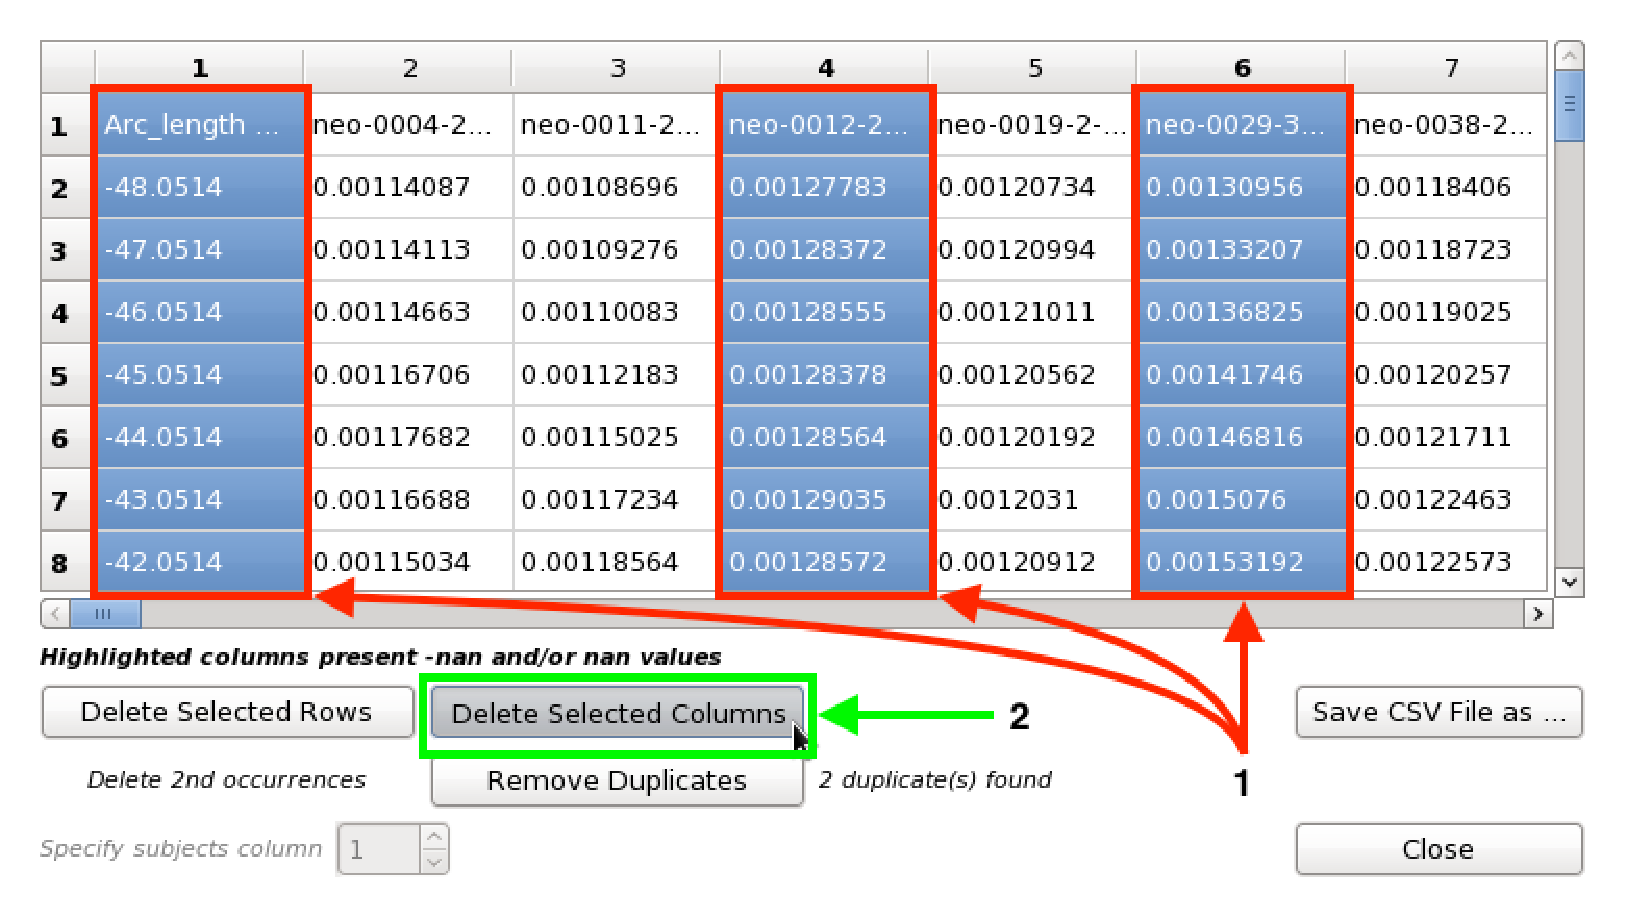
\includegraphics[width=\textwidth]{deleteColumnsOut.eps}
		\caption{Data selection.}
		\label{fig:deleteColumnsOut}
	\end{subfigure}

	\begin{subfigure}{0.45\textwidth}
    	\includegraphics[width=\textwidth]{searchSubject1Out.eps}
		\caption{Subjects QC}
		\label{fig:subjectsTab_filed}
	\end{subfigure}	
	\begin{subfigure}{0.45\textwidth}
    	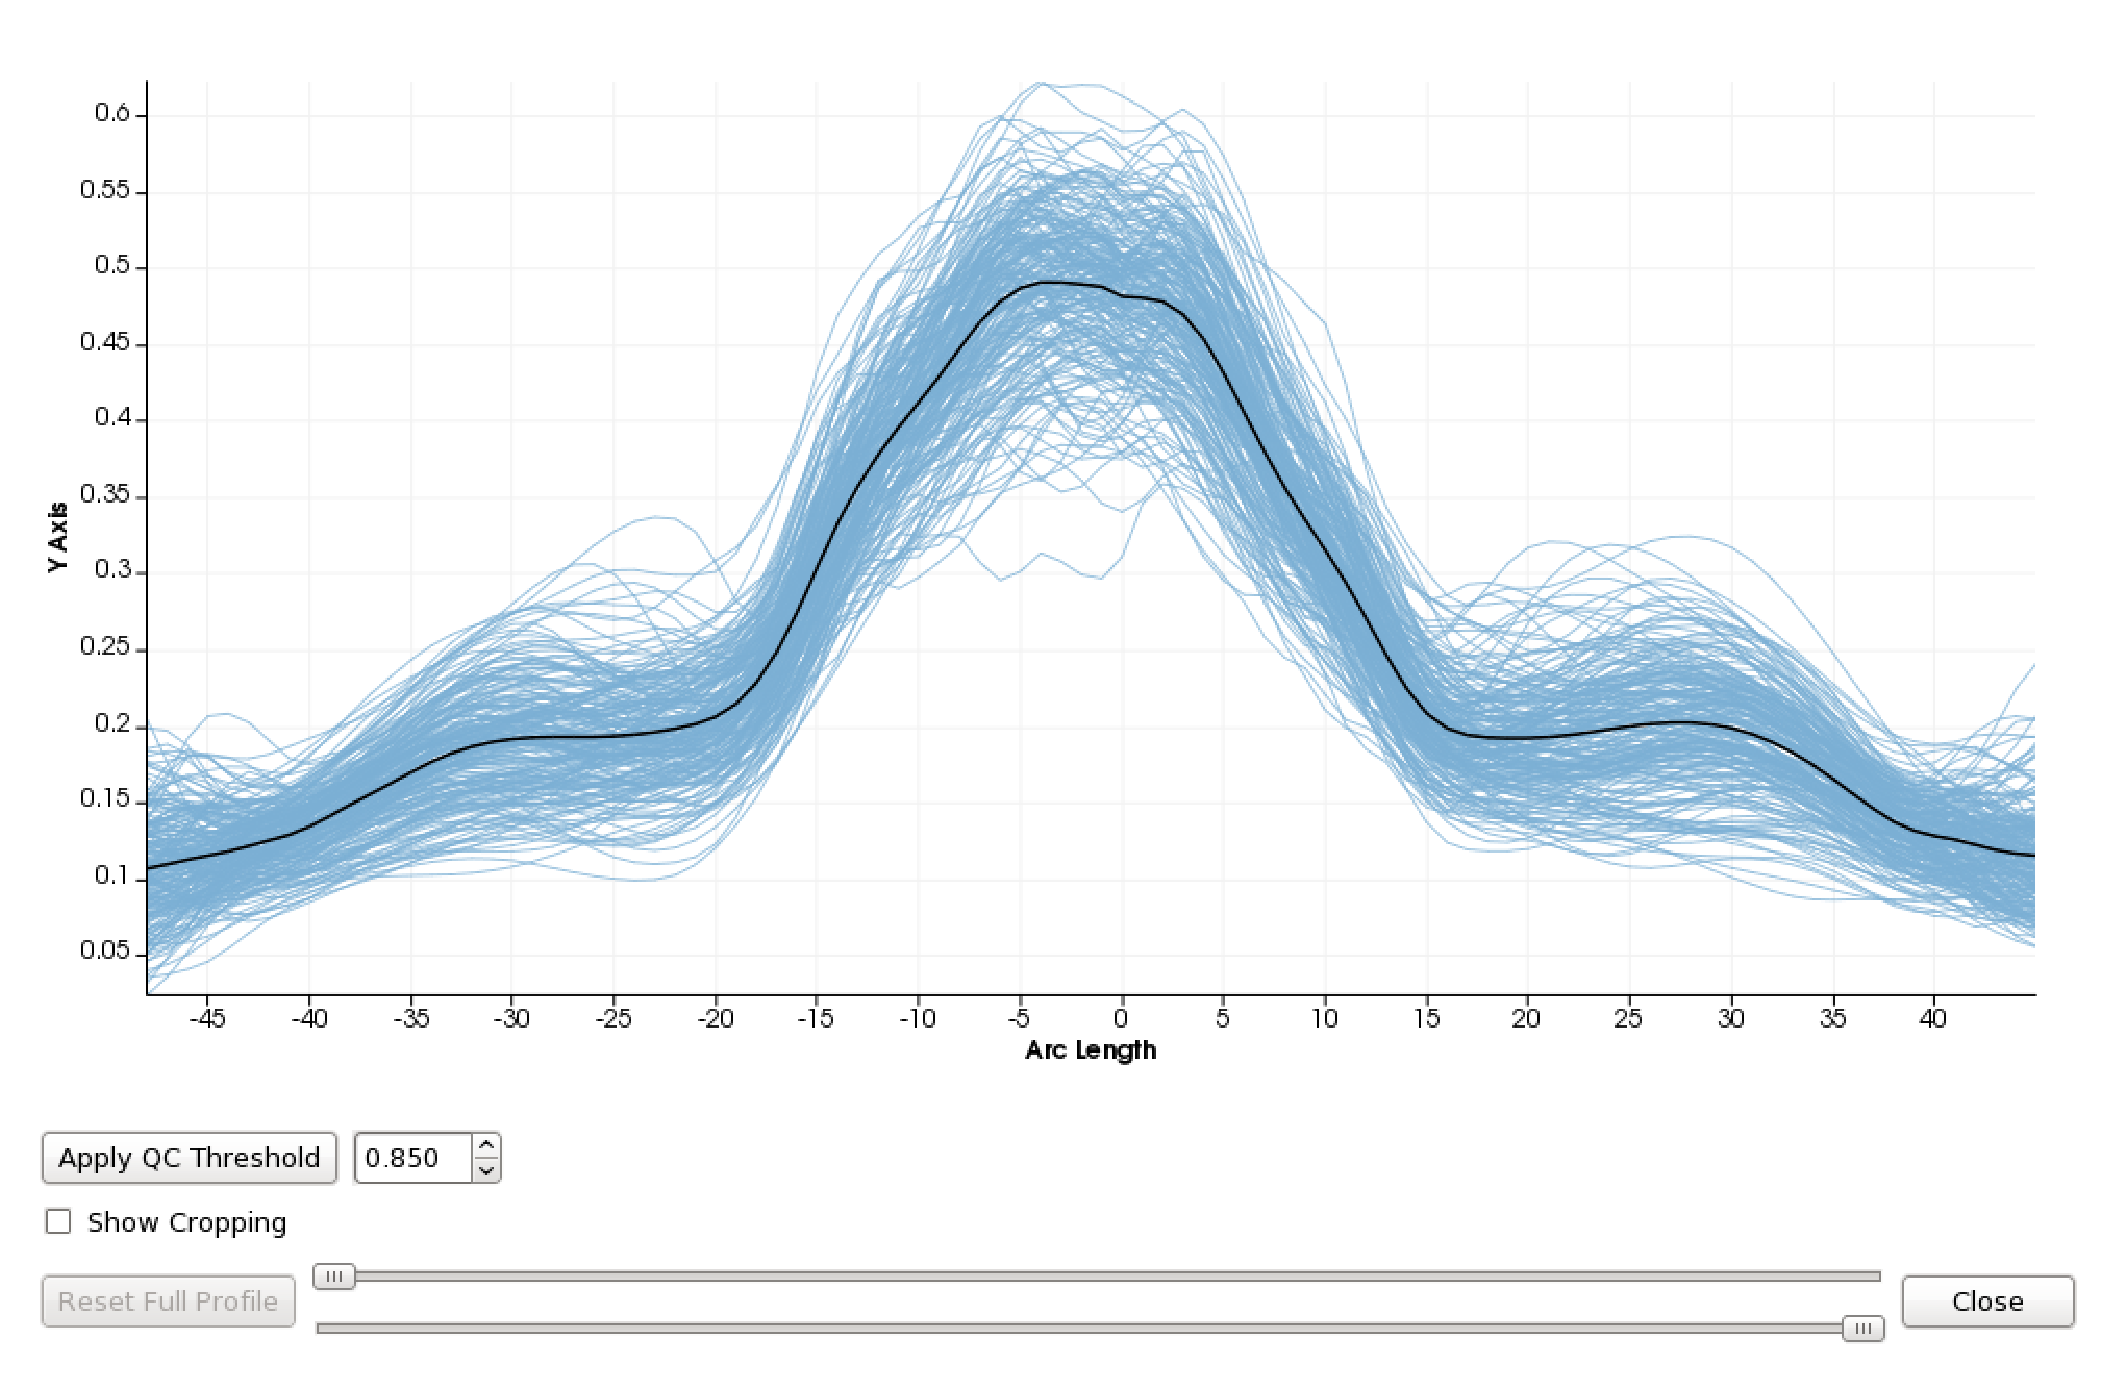
\includegraphics[width=\textwidth]{applyQC1Out.eps}
    	\caption{Fibers QC}
    	\label{fig:applyQC1}
	\end{subfigure}

	\begin{subfigure}{0.45\textwidth}
    	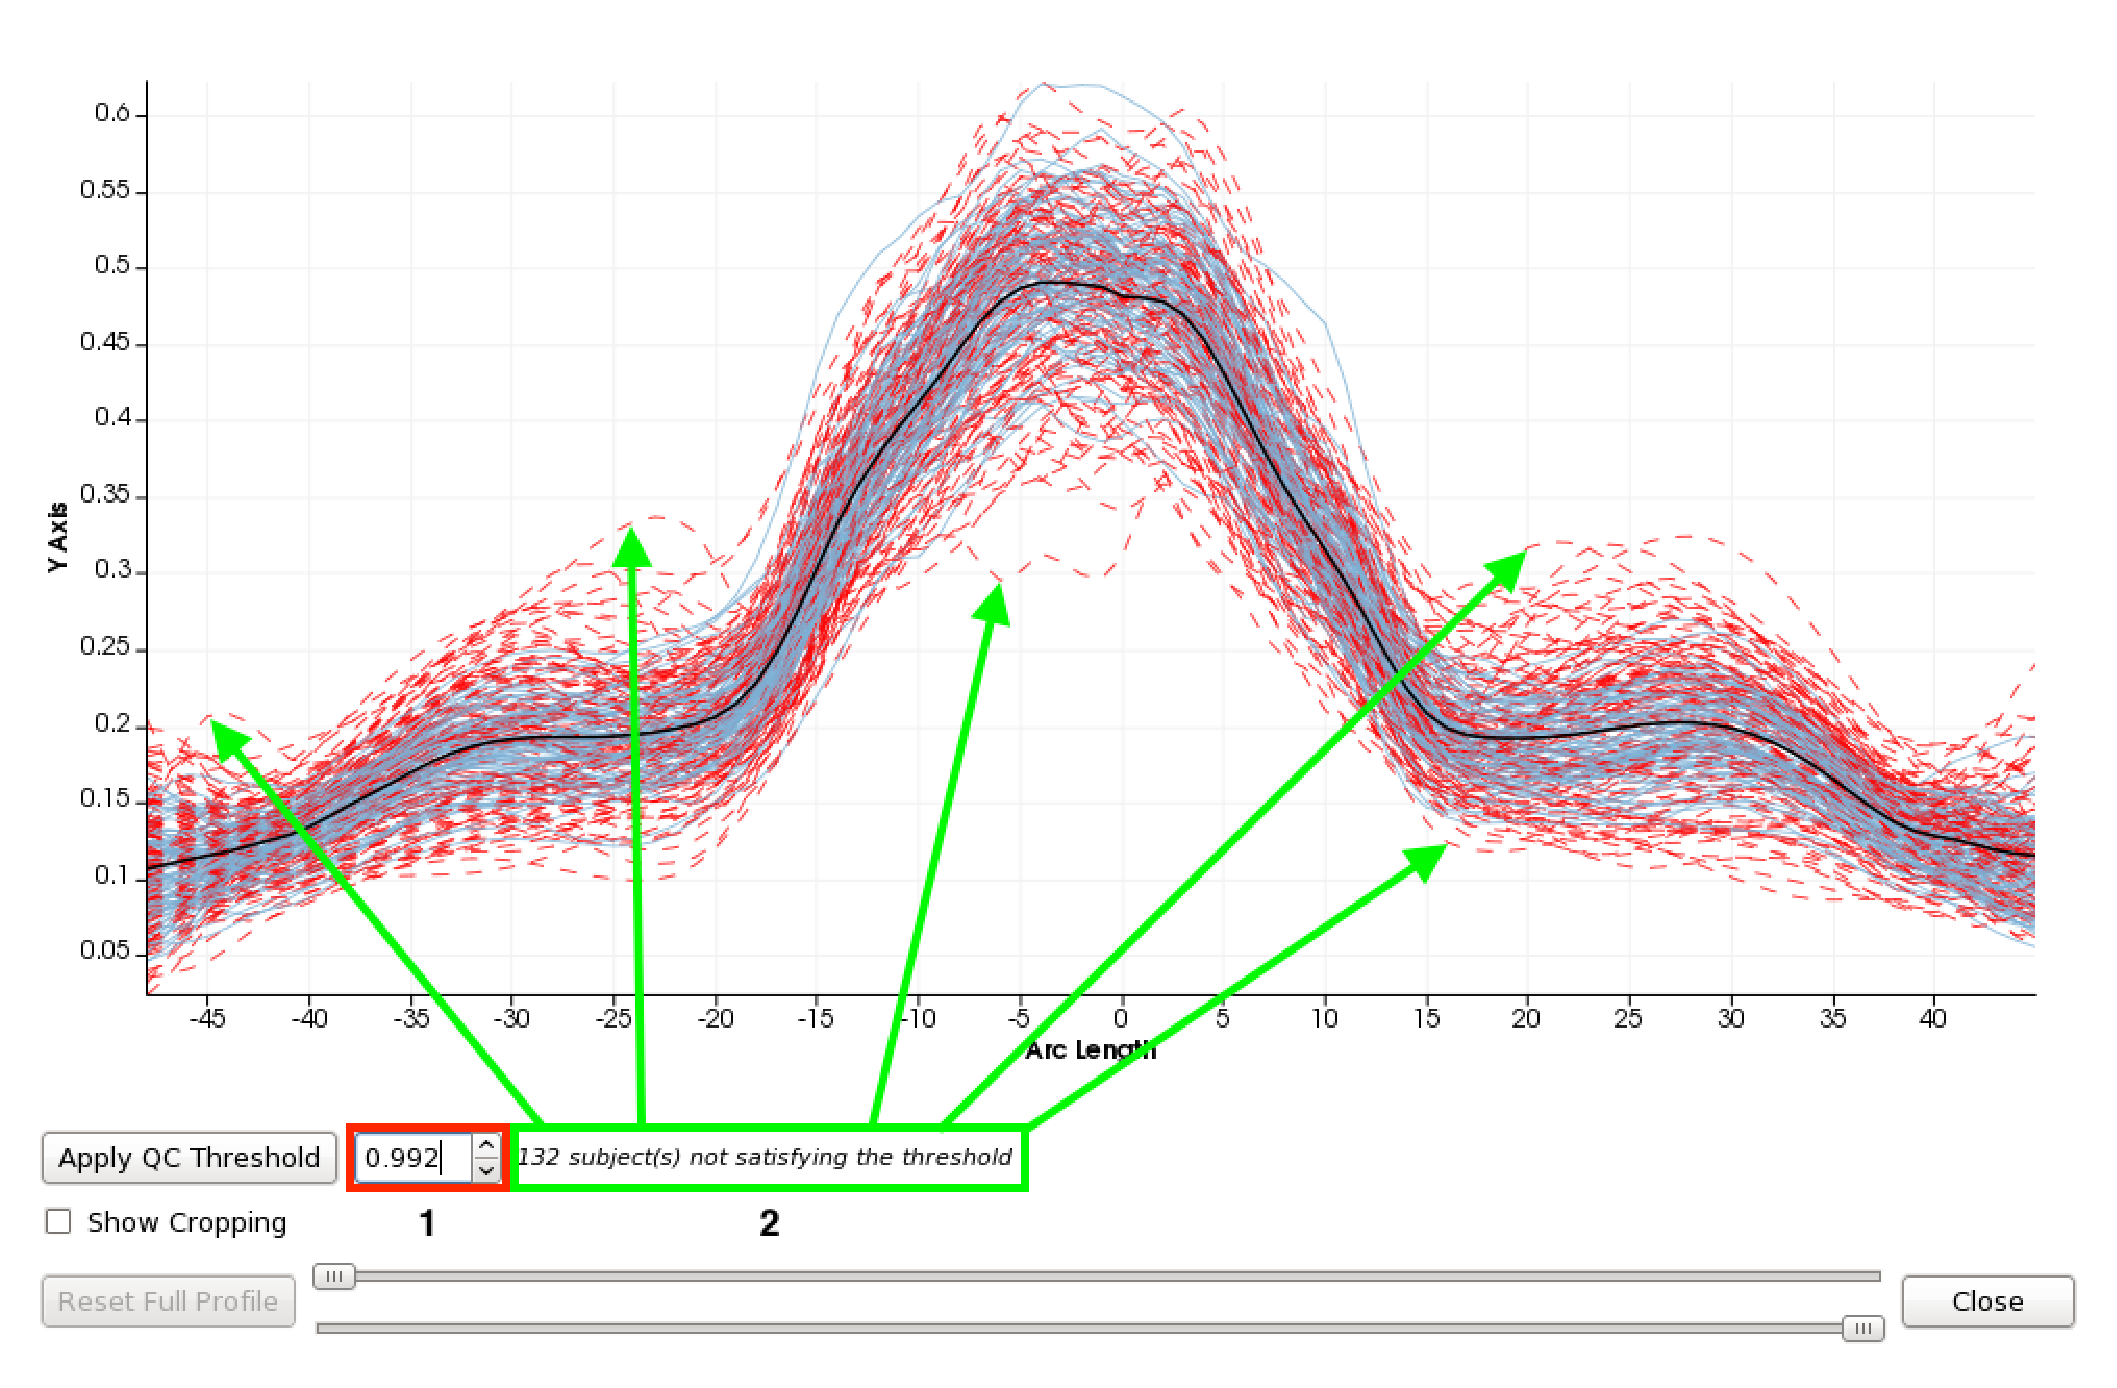
\includegraphics[width=\textwidth]{applyQC2Out.eps}
    	\caption{Fibers QC}
    	\label{fig:applyQC2}
	\end{subfigure}
	\begin{subfigure}{0.45\textwidth}
		\includegraphics[width=\textwidth]{runFADTTSterOut.eps}
		\caption{Execution}
		\label{fig:executionTab}
	\end{subfigure}

	\caption[Setting inputs]{ 
	a) Add input files and check if they are valid. Choose covariates of interest. 
	b) Delete subjects from the study. 
	c) Select subjects matched across all input files provided.
	d) Fibers are shown in blue, mean fiber is shown in bold. 
	e) Red fibers do not pass the QC threshold applied. The fiber bundles may also be cropped at the beginning or the end.
	f) \textit{Matlab} script generation and running FADTTS tool box.}
	\label{fig:FADTTSterApp}
\end{figure} 

\begin{figure}
	\centering
	\begin{subfigure}{0.45\textwidth}
		\includegraphics[width=\textwidth]{RawDataOut.eps}
	   	\caption{Raw data}
	   	\label{fig:RawData}
	\end{subfigure}
	\begin{subfigure}{0.45\textwidth}
		\includegraphics[width=\textwidth]{RawStatsOut.eps}
	   	\caption{Raw statistics}
	   	\label{fig:RawStats}
	\end{subfigure}

	\begin{subfigure}{0.45\textwidth}
		\includegraphics[width=\textwidth]{RawBetasPropOut.eps}
	   	\caption{Raw betas by properties}
	   	\label{fig:RawBetasProp}
	\end{subfigure}
	\begin{subfigure}{0.45\textwidth}
		\includegraphics[width=\textwidth]{RawBetasCovOut.eps}
	   	\caption{Raw betas by covariates}
	   	\label{fig:RawBetasCov}
	\end{subfigure}

	\begin{subfigure}{0.45\textwidth}
		\includegraphics[width=\textwidth]{omnibusLpOut.eps}
	   	\caption{Omnibus local p values}
	   	\label{fig:omnibusLp}
	\end{subfigure}
	\begin{subfigure}{0.45\textwidth}
		\includegraphics[width=\textwidth]{omnibusFDRLpOut.eps}
	   	\caption{Omibus FDR local p values}
	   	\label{fig:omnibusFDRLp}
	\end{subfigure}

	\label{fig:rawomnibus}
	\caption{Plotting raw data and raw statistics with properties such as AD and covariates such as gender.
	The properties and covariates may be optional depending on the plot.
	Figures \ref{fig:omnibusLp} and \ref{fig:omnibusFDRLp} shows the local p values and false discovery rate (FDR) for 
	different characteristics.}
\end{figure}

\begin{figure}
	\centering
	\begin{subfigure}{0.45\textwidth}
		\includegraphics[width=\textwidth]{omnibusFDRSigBetasPropOut.eps}
	   	\caption{Omnibus FDR significant betas by properties}
	   	\label{fig:omnibusFDRSigBetasTab}
	\end{subfigure}
	\begin{subfigure}{0.45\textwidth}
		\includegraphics[width=\textwidth]{omnibusFDRSigBetasCovOut.eps}
	   	\caption{Omnibus FDR significant betas by covariate}
	   	\label{fig:omnibusFDRSigBetasCov}
	\end{subfigure}

	\begin{subfigure}{0.45\textwidth}
		\includegraphics[width=\textwidth]{omnibusBetasConfBandsOut.eps}
	   	\caption{Omnibus betas with confidence bands}
	   	\label{fig:omnibusBetasConfBands}
	\end{subfigure}
	\begin{subfigure}{0.45\textwidth}
		\includegraphics[width=\textwidth]{phFDRSigBetasAvg1Out.eps}
	   	\caption{Post-Hoc FDR significant Betas on average raw data}
	   	\label{fig:phFDRSigBetasAvg1}
	\end{subfigure}

	\begin{subfigure}{0.45\textwidth}
		\includegraphics[width=\textwidth]{phFDRSigBetasPropOut.eps}
	   	\caption{Post-Hoc FDR significant betas by properties}
	   	\label{fig:phFDRSigBetasProp}
	\end{subfigure}
	\begin{subfigure}{0.45\textwidth}
		\includegraphics[width=\textwidth]{phFDRLpCovOut.eps}
	   	\caption{Post-Hoc FDR significant local p values by covariates}
	   	\label{fig:phFDRLpCov}
	\end{subfigure}
	
	\caption{Figures \ref{fig:omnibusFDRSigBetasTab} and \ref{fig:omnibusFDRSigBetasCov} 
	shows omnibus plots false discovery rate (FDR) significant type II errors for 
	properties and covariates. Figures \ref{fig:phFDRSigBetasAvg1} and \ref{fig:phFDRSigBetasProp} 
	allows visualizing the post-hoc FDR for a property and a covariate.
	Significant betas are overlay in each line.}
	\label{fig:omnibusph}
\end{figure}

% \begin{figure}
% 	\centering
% 	\includegraphics[width=0.8\textwidth]{phFDRSigBetasCovOut.eps}
%    	\caption{}
%    	\label{fig:phFDRSigBetasCov}
% \end{figure}

\section{CONCLUSION} 
\label{sec:CONCLUSION}

FADTTS is a novel tool to delineate several diffusion properties along major WM bundles and association with 
a set of covariates of interest. To use this tool the user is required to know scripting languages. 

The first contribution presented in this paper is to enable FADTTS to non-technical users. 
Granting access to the sophisticated statistical analysis available in FADTTS.
The tool guides users through 
a series of steps which simplifies setting up FADTTS. 
FADTTSter is actively being used by researchers at the University of North Carolina. 

The second contribution presented here is the new set of interactive plots. 
FADTTS outputs may be difficult to understand with out having the possibility to drill down 
on the raw data and statistics. We have shown several plots that 
will enhance the researcher's capability to understand the results.

By enabling FADTTS to a broader audience, we seek to accelerate hypothesis testing in neuroimaging studies involving
heterogeneous clinical data and diffusion tensor imaging.
We expect that this novel tool will lead to new findings in our clinical applications.

This work is submitted to the Biomedical Applications in Molecular, Structural, and Functional Imaging conference. 
The source code of this application is available in NITRC\footnote{\url{http://www.nitrc.org/namicdtifiber/}}.

\acknowledgments
\label{sec:acknowledgments}

We would like to thank Jessica Bullins and Shaili Jha for their valuable feedback during the development 
of this application. 

%%%%%%%%%%%%%%%%%%%%%%%%%%%%%%%%%%%%%%%%%%%%%%%%%%%%%%%%%%%%%
%%%%% References %%%%%

\bibliography{FADTTSter_article}   %>>>> bibliography data in report.bib
\bibliographystyle{spiebib}   %>>>> makes bibtex use spiebib.bst

\end{document} 
